\section{Occupant Thermal Comfort }\label{occupant-thermal-comfort}

The integration of a sophisticated building thermal analysis tool with thermal comfort models allows one to perform an energy analysis on a zone and simultaneously determine if the environmental control strategy will be sufficient for the occupants to be thermally comfortable. This section is intended to provide background on thermal comfort, present an overview of state of the art thermal comfort models, and present the mathematical models that have been incorporated into EnergyPlus.

Thermal comfort modeling in EnergyPlus is controlled primarily by the People input object. This includes input for selecting the type of thermal comfort model that is desired by the user as well as parameters that serve as inputs to the thermal comfort models. These parameters include the activity level, the work efficiency, the air velocity and the clothing insulation level for people within the space. All four of these parameters can be scheduled. More information on the People input object can be found in the EnergyPlus Input/Output Reference. More information on how each of these parameters is used and the specific modeling equations for the thermal comfort models can be found below.

\subsection{Background on Thermal Comfort Models}\label{background-on-thermal-comfort-models}

Throughout the last few decades, researchers have been exploring the thermal, physiological and psychological response of people in their environment in order to develop mathematical models to predict these responses. Researchers have empirically determined building occupants' thermal responses to the combined thermal effect of the personal, environmental and physiological variables that influence the condition of thermal comfort.

There are two personal variables that influence the condition of thermal comfort: the thermal resistance of the clothing (I\(_{cl}\)), and the metabolic rate (H/A\(_{Du}\)).

The thermal resistance of the clothing (I\(_{cl}\)) is measured in units of ``clo.'' The 1985 ASHRAE Handbook of Fundamentals (ASHRAE 1985) suggests multiplying the summation of the individual clothing items clo value by a factor of 0.82 to determine the overall clo value for clothing ensembles.

The metabolic rate (H/A\(_{Du}\)) is a measure of the internal heat production rate of an occupant (H) in W/hr per unit of ``Dubois'' body surface area (A\(_{Du}\)) in units of m\(^{2}\). The DuBois body surface area is given by:

\begin{equation}
{A_{Du}} = 0.202{(weight)^{0.425}}{(height)^{0.725}}
\end{equation}

Using this equation, an area of 1.8 m\(^{2}\) represents the surface area of an average person of weight 70 kg and height 1.73 m (Fanger 1967).  In EnergyPlus, this average person area of 1.8 m\(^{2}\) is used for the body surface area all thermal comfort models.  The metabolic rate is measured in mets, where 1 met = 58.2 W/m\(^{2}\).

The environmental variables that influence the conditions of thermal comfort include:

\begin{enumerate}
\def\labelenumi{(\arabic{enumi})}
\item
  Air Temperature (T\(_{a}\)),
\item
  Mean Radiant Temperature (T\(_{r}\)),
\item
  Relative air velocity (v),
\item
  Water vapor pressure in ambient air (P\(_{a}\)).
\end{enumerate}

The Air Temperature (T\(_{a}\)), a direct environmental index, is the dry-bulb temperature of the environment. It is calculated using either the mean air temperature for the zone in question or the air temperature calculated by some of the more detailed zone air models available in EnergyPlus. The Mean Radiant Temperature (T\(_{r}\)) is a rationally derived environmental index defined as the uniform black-body temperature that would result in the same radiant energy exchange as in the actual environment. This value can be calculated in several ways as outlined in the Mean Radiant Temperature Calculation section later in this document.  The Relative air velocity (v) a direct environmental index is a measure of the air motion obtainable via a hot wire or vane anemometers. The Water vapor pressure in ambient air (P\(_{a}\)) is a direct environmental index.

The physiological variables that influence the conditions of thermal comfort include:

\begin{enumerate}
\def\labelenumi{(\arabic{enumi})}
\item
  Skin Temperature (T\(_{sk}\)),
\item
  Core or Internal Temperature (T\(_{cr}\)),
\item
  Sweat Rate,
\item
  Skin Wettedness (w),
\item
  Thermal Conductance (K) between the core and skin.
\end{enumerate}

where the Skin Temperature (T\(_{sk}\)), the Core Temperature (T\(_{cr}\)) and the Sweat Rate are physiological indices. The Skin Wettedness (w) is a rationally derived physiological index defined as the ratio of the actual sweating rate to the maximum rate of sweating that would occur if the skin were completely wet.

One more consideration is important in dealing with thermal comfort - the effect of asymmetrical heating or cooling. This could occur when there is a draft or when there is a radiant flux incident on a person (which is what is of primary interest to us here). Fanger (1967) noted that the human regulatory system is quite tolerant of asymmetrical radiant flux. A reasonable upper limit on the difference in mean radiant temperature (T\(_{r}\)) from one direction to the opposing direction is 15\(^{\circ}\)C. (ASHRAE 1984). This limit is lower if there is a high air velocity in the zone.

% table 78
\begin{longtable}[c]{p{1.2in}p{2.0in}p{0.8in}p{0.8in}p{1.2in}}
\caption{General Nomenclature list for Thermal Comfort Models \label{table:general-nomenclature-list-for-thermal-comfort}} \tabularnewline
\toprule 
Mathematical variable & Description & Units ~ & Range & Source Code Variable \tabularnewline
\midrule
\endfirsthead

\caption[]{General Nomenclature list for Thermal Comfort Models} \tabularnewline
\toprule 
Mathematical variable & Description & Units ~ & Range & Source Code Variable \tabularnewline
\midrule
\endhead

A\(_{Du}\) & Dubois body surface area & m\(^{2}\) & - & - \tabularnewline
H & Internal heat production rate of an occupant per unit area = M – W & W/m\(^{2}\) & - & IntHeatProd \tabularnewline
I\(_{cl}\) & Thermal resistance of the clothing & clo & - & CloUnit \tabularnewline
M & Metabolic rate per unit area & W/m\(^{2}\) & - & ActLevel \tabularnewline
P\(_{a}\) & Water vapor pressure in ambient air & Torr & - & VapPress \tabularnewline
T\(_{a}\) & Air temperature & \(^{\circ}\)C & - & AirTemp \tabularnewline
T\(_{cr}\) & Core or internal temperature & \(^{\circ}\)C & - & CoreTemp \tabularnewline
T\(_{r}\) & Mean radiant temperature & \(^{\circ}\)C & - & RadTemp \tabularnewline
T\(_{sk}\) & Skin temperature & \(^{\circ}\)C & - & - \tabularnewline
v & Relative air velocity & m/s & - & AirVel \tabularnewline
W & The rate of heat loss due to the performance of work & W/m\(^{2}\) & - & WorkEff \tabularnewline
w & Skin wettedness & - & - & - \tabularnewline
\bottomrule
\end{longtable}

\subsection{Mathematical Models for Predicting Thermal Comfort}\label{mathematical-models-for-predicting-thermal-comfort}

Many researchers have been exploring ways to predict the thermal sensation of people in their environment based on the personal, environmental and physiological variables that influence thermal comfort. From the research done, some mathematical models that simulate occupants' thermal response to their environment have been developed. Most thermal comfort prediction models use a seven or nine point thermal sensation scale, as in the following tables.

% table 79
\begin{longtable}[c]{@{}ll@{}}
\caption{Seven point Thermal Sensation Scale \label{table:seven-point-thermal-sensation-scale}} \tabularnewline
\toprule 
Sensation & Description \tabularnewline
\midrule
\endfirsthead

\caption[]{Seven point Thermal Sensation Scale} \tabularnewline
\toprule 
Sensation & Description \tabularnewline
\midrule
\endhead

3 & Hot \tabularnewline
2 & Warm \tabularnewline
1 & slightly warm \tabularnewline
0 & neutral \tabularnewline
-1 & slightly cool \tabularnewline
-2 & cool \tabularnewline
-3 & cold \tabularnewline
\bottomrule
\end{longtable}

% table 80
\begin{longtable}[c]{@{}ll@{}}
\caption{Nine point Thermal Sensation Scale \label{table:nine-point-thermal-sensation-scale}} \tabularnewline
\toprule 
Sensation Value & Description \tabularnewline
\midrule
\endfirsthead

\caption[]{Nine point Thermal Sensation Scale} \tabularnewline
\toprule 
Sensation Value & Description \tabularnewline
\midrule
\endhead

4 & very hot \tabularnewline
3 & hot \tabularnewline
2 & warm \tabularnewline
1 & slightly warm \tabularnewline
0 & neutral \tabularnewline
-1 & slightly cool \tabularnewline
-2 & cool \tabularnewline
-3 & cold \tabularnewline
-4 & very cold \tabularnewline
\bottomrule
\end{longtable}

The most notable models have been developed by P.O. Fanger (the Fanger Comfort Model), the J. B. Pierce Foundation (the Pierce Two-Node Model), and researchers at Kansas State University (the KSU Two-Node Model). Berglund (1978) presents a detailed description of the theory behind these three models.

Note for all Thermal Comfort reporting:~ Though the published values for thermal comfort ``vote'' have a discrete scale (e.g. --3 to +3 or --4 to +4), the calculations in EnergyPlus are carried out on a continuous scale and, thus, reporting may be ``off the scale'' with specific conditions encountered in the space.~ This is not necessarily an error in EnergyPlus -- rather a different approach that does not take the ``limits'' of the discrete scale values into account.

The main similarity of the three models is that all three apply an energy balance to a person and use the energy exchange mechanisms along with experimentally derived physiological parameters to predict the thermal sensation and the physiological response of a person due to their environment. The models differ somewhat in the physiological models that represent the human passive system (heat transfer through and from the body) and the human control system (the neural control of shivering, sweating and skin blood flow). The models also differ in the criteria used to predict thermal sensation. However, all three models use information from the People statement and the thermal comfort model is selected via the People statement in a user's input file. Scheduled parameters such as the activity level, work efficiency, air velocity, and clothing insulation level all have a direct bearing on the thermal comfort models. For more information on the input of these parameters, see the People statement in the EnergyPlus Input/Output Reference. For more information on how each individual thermal comfort model uses these parameters, please consult the next several sections.

\subsection{Fanger Comfort Model}\label{fanger-comfort-model}

Fanger's Comfort model was the first human comfort model that was developed. It was first published in 1967 (Fanger 1967), then updated in 1970 (Fanger 1970), and helped set the stage for the Pierce and KSU models. The mathematical model developed by P.O. Fanger is probably the most well known of the three models and is the easiest to use because it has been put in both chart and graph form.

\subsubsection{Fanger Model Nomenclature List}\label{fanger-model-nomenclature-list}

% table 81
\begin{longtable}[c]{p{1.2in}p{2.0in}p{0.8in}p{0.8in}p{1.2in}}
\caption{Nomenclature list for Fanger model \label{table:nomenclature-list-for-fanger-model}} \tabularnewline
\toprule 
Mathematical variable & Description & Units & Range & Source Code Variable \tabularnewline
\midrule
\endfirsthead

\caption[]{Nomenclature list for Fanger model} \tabularnewline
\toprule 
Mathematical variable & Description & Units & Range & Source Code Variable \tabularnewline
\midrule
\endhead

A\(_{Du}\) & Dubois body surface area & m\(^{2}\) & - & BodySurfaceArea \tabularnewline
C\(_{res}\) & The rate of dry respiratory heat loss & W/m\(^{2}\) & - & DryRespHeatLoss \tabularnewline
E\(_{dif}\) & The rate of heat loss from the diffusion of water vapor through the skin & W/m\(^{2}\) & - & EvapHeatLossDiff \tabularnewline
E\(_{res}\) & The rate of latent respiratory heat loss & W/m\(^{2}\) & - & LatRespHeatLoss \tabularnewline
E\(_{rsw,req}\) & The rate of heat loss from the evaporation of regulatory sweating at the state of comfort & W/m\(^{2}\) & - & EvapHeatLossRegComf \tabularnewline
E\(_{sk}\) & Total evaporative heat loss from skin & W/m\(^{2}\) & ~ & EvapHeatLoss \tabularnewline
f\(_{cl}\) & The ratio of clothed body & - & ~ & CloBodyRat \tabularnewline
f\(_{eff}\) & The fraction of surface effective for radiation ( = 0.72) & - & - & RadSurfEff \tabularnewline
H & Internal heat production rate of an occupant per unit area ( = M – W) & W/m\(^{2}\) & - & IntHeatProd \tabularnewline
h\(_{c}\) & Convective heat transfer coefficient & W/m\(^{2}\)-\(^{\circ}\)C & - & Hc \tabularnewline
L & All the modes of energy loss from body & W/m\(^{2}\) & - & - \tabularnewline
M & Metabolic rate per unit area & W/m\(^{2}\) & - & ActLevel \tabularnewline
P\(_{a}\) & Water vapor pressure in ambient air & Torr & - & VapPress \tabularnewline
PMV & Predicted Mean Vote & - & (-4)-4 & PMV \tabularnewline
PPD & Predicted Percentage of Dissatisfied & - & 0-100 & PPD \tabularnewline
Q\(_{c}\) & The rate of convective heat loss & W/m\(^{2}\) & - & ConvHeatLoss \tabularnewline
Q\(_{dry}\) & Sensible heat flow from skin & W/m\(^{2}\) & ~ & DryHeatLoss \tabularnewline
Q\(_{r}\) & The rate of radiative heat loss & W/m\(^{2}\) & - & RadHeatLoss \tabularnewline
Q\(_{res}\) & The rate of respiratory heat loss & W/m\(^{2}\) & - & RespHeatLoss \tabularnewline
T\(_{a}\) & Air temperature & \(^{\circ}\)C & - & AirTemp \tabularnewline
T\(_{cl}\) & Clothing surface temperature & \(^{\circ}\)C & - & CloSurfTemp \tabularnewline
T\(_{cla}\) & Clothing surface temperature (Absolute) & K & - & AbsCloSurfTemp \tabularnewline
T\(_{ra}\) & Mean radiant temperature & K & - & AbsRadTemp \tabularnewline
W & The rate of heat loss due to the performance of work & W/m\(^{2}\) & - & WorkEff \tabularnewline
$\varepsilon$ & The emissivity of clothing-skin surface & - & - & SkinEmiss \tabularnewline
$\sigma$ & The Stefan-Boltzman constant ( = 5.67×10\(^{-8}\)) & W/m\(^{2}\)K\(^{4}\) & - & StefanBoltz \tabularnewline
\bottomrule
\end{longtable}

\subsubsection{Description of the model and algorithm}\label{description-of-the-model-and-algorithm}

Fanger developed the model based on the research he performed at Kansas State University and the Technical University of Denmark. Fanger used the seven-point form of a thermal sensation scale along with numerous experiments involving human subjects in various environments. He related the subjects' response to various environmental variables which influence the condition of thermal comfort. Fanger's model is based upon an energy analysis that takes into account all the modes of energy loss (L) from the body, including: the convection and radiant heat loss from the outer surface of the clothing, the heat loss by water vapor diffusion through the skin, the heat loss by evaporation of sweat from the skin surface, the latent and dry respiration heat loss and the heat transfer from the skin to the outer surface of the clothing. The model assumes that the person is thermally at steady state with the interior environment.

\begin{equation}
M = L
\end{equation}

\begin{equation}
L = {Q_{res}} + {Q_{dry}} + {E_{sk}}
\end{equation}

\begin{equation}
{Q_{res}} = {E_{res}} + {C_{res}} = 0.000017M(5867 - {P_a}) + 0.0014M(34 - {T_a})
\end{equation}

In the EnergyPlus source code,  Q\(_{res}\), E\(_{res}\) and C\(_{res}\) are calculated using the following equations, respectively:

RespHeatLoss = LatRespHeatLoss + DryRespHeatLoss

LatRespHeatLoss = 0.000017*ActLevel*(5867. - VapPress)

DryRespHeatLoss = 0.0014*ActLevel*(34.- AirTemp)

\begin{equation}
{Q_{dry}} = {Q_c} + {Q_r}
\end{equation}

\begin{equation}
{Q_c} = {h_c} \times {f_{cl}}({T_{cl}} - {T_a})
\end{equation}

\begin{equation}
{Q_{r}}=3.96*f\left(_{l}\right)*{[}(0.01*T\left(_{a}\right))\left(^{4}\right)-(0.01*T\left(_{a}\right))\left(^{4}\right){]}
\label{eq:FangerQr}
\end{equation}

In the EnergyPlus source code, Q\(_{dry}\), Q\(_{c}\) and Q\(_{r}\) are calculated using the following equations, respectively:

DryHeatLoss = ConvHeatLoss + RadHeatLoss

ConvHeatLos = CloBodyRat*Hc*(CloSurfTemp - AirTemp)

RadHeatLoss = 3.96*CloBodyRat*{[}(0.01*AbsCloSurfTemp)**4 - (0.01*AbsRadTemp)**4{]}

\begin{equation}
{E_{rsw}} = 0.42(H - 58.2)~~~~for~\left(H > 58.2\right)
\end{equation}

\begin{equation}
{E_{rsw}} = 0~~~~for~\left(H \le 58.2\right)
\end{equation}

\begin{equation}
{E_{f}}=0.00305*(5733.0-6.99H-P_{a})
\end{equation}

\begin{equation}
{E_{sk}} = {E_{rsw}} + {E_{diff}}
\end{equation}

In the EnergyPlus source code, E\(_{rsw}\), E\(_{f}\) and E\(_{sk}\) are calculated using the following equations, respectively:

EvapHeatLossRegComf = 0.42*(IntHeatProd - ActLevelConv) or 0.0 depending on H value

EvapHeatLossDiff = 0.00305*(5733.0 - 6.99*IntHeatProd - VapPress)

EvapHeatLoss = EvapHeatLossRegComf + EvapHeatLossDiff

The Fanger model was developed using the thermal sensation votes from subjects at KSU and in Denmark, and the Predicted Mean Vote (PMV) thermal sensation scale is based on how the energy loss (L) deviates from the metabolic rate (M) in the following form:

\begin{equation}
PMV = (0.303{e^{ - 0.036M}} + 0.028)(H - L)
\end{equation}

In the EnergyPlus source code, PMV is calculated using the following equations in conjunction with the equations shown above:

PMV = ThermSensTransCoef*(IntHeatProd - EvapHeatLoss - RespHeatLoss - DryHeatLoss)

ThermSensTransCoef = 0.303*EXP(-0.036*ActLevel) + 0.028

IntHeatProd = ActLevel - WorkEff

Predicted Percent of Dissatisfied (PPD) people at each PMV is calculated as follows:

\begin{equation}
PPD = 100.0 - 95.0*EXP(-0.03353{PMV^{4}} - 0.2179{PMV^{2}})
\end{equation}

\subsection{Pierce Two-Node Model}\label{pierce-two-node-model}

The Pierce Two-Node model was developed at the John B. Pierce Foundation at Yale University. The model has been continually expanding since its first publication in 1970 (Gagge et.al. 1970). The most recent version on the model appears in the 1986 ASHRAE Transactions (Gagge et.al. 1986).

\subsubsection{Pierce Two-Node Model Nomenclature List}\label{pierce-two-node-model-nomenclature-list}

% table 82
\begin{longtable}[c]{p{1.2in}p{2.0in}p{0.8in}p{0.8in}p{1.2in}}
\caption{Nomenclature list for Pierce Two-Node model \label{table:nomenclature-list-for-pierce-two-node-model}} \tabularnewline
\toprule 
Mathematical variable & Description & Units ~ & Range & Source Code Variable \tabularnewline
\midrule
\endfirsthead

\caption[]{Nomenclature list for Pierce Two-Node model} \tabularnewline
\toprule 
Mathematical variable & Description & Units ~ & Range & Source Code Variable \tabularnewline
\midrule
\endhead

C\(_{dil}\) & Constant for skin blood flow & ~ & ~ & SkinBloodFlowConst \tabularnewline
C\(_{res}\) & The rate of dry respiratory heat loss & W/m\(^{2}\) & - & DryRespHeatLoss \tabularnewline
C\(_{sw}\) & Proportionality constant for sweat control & g/m\(^{2}\)hr & ~ & SweatContConst \tabularnewline
DISC & Predicted discomfort vote & - & (-5)-5 & DISC \tabularnewline
E\(_{dif}\) & The rate of heat loss from the diffusion of water vapor through the skin & W/m\(^{2}\) & - & EvapHeatLossDiff \tabularnewline
E\(_{max}\) & Maximum evaporative heat loss & W/m\(^{2}\) & ~ & EvapHeatLossMax \tabularnewline
E\(_{sk}\) & Total evaporative heat loss from skin & W/m\(^{2}\) & ~ & EvapHeatLoss \tabularnewline
E\(_{res}\) & The rate of latent respiratory heat loss & W/m\(^{2}\) & - & LatRespHeatLoss \tabularnewline
E\(_{rsw}\) & The rate of heat loss from the evaporation of regulatory sweating & W/m\(^{2}\) & - & EvapHeatLossRegSweat \tabularnewline
E\(_{rsw,req}\) & The rate of heat loss from the evaporation of regulatory sweating at the state of comfort & W/m\(^{2}\) & ~ & EvapHeatLossRegComf \tabularnewline
ET* & Effective Temperature & \(^{\circ}\)C & - & ET \tabularnewline
f\(_{cl}\) & The ratio of clothed body & - & ~ & CloBodyRat \tabularnewline
f\(_{eff}\) & The fraction of surface effective for radiation ( = 0.72) & - & - & RadSurfEff \tabularnewline
H & Internal heat production rate of an occupant per unit area ( = M – W) & W/m\(^{2}\) & - & IntHeatProd \tabularnewline
h & Combined heat transfer coefficient & W/m\(^{2}\)-\(^{\circ}\)C & ~ & H \tabularnewline
h\(_{c}\) & Convective heat transfer coefficient & W/m\(^{2}\)-\(^{\circ}\)C & - & Hc \tabularnewline
h\(_{e}\)’ & Combined evaporative heat transfer coefficient & W/(m\(^{2}\)kP\(_{a}\)) & ~ & - \tabularnewline
h\(_{r}\) & Radiant heat transfer coefficient & W/m\(^{2}\)-\(^{\circ}\)C & - & Hr \tabularnewline
I\(_{cl}\) & Clothing insulation & m\(^{2}\)\(^{\circ}\)C/W & ~ & - \tabularnewline
L & All the modes of energy loss from body & W/m\(^{2}\) & - & - \tabularnewline
L\(_{ET*}\) & All the modes of energy loss from body at ET* & W/m\(^{2}\) & ~ & - \tabularnewline
L\(_{SET*}\) & All the modes of energy loss from body at SET* & W/m\(^{2}\) & ~ & - \tabularnewline
M & Metabolic rate per unit area & W/m\(^{2}\) & - & ActLevel \tabularnewline
M\(_{act}\) & Metabolic heat production due to activity & W/m\(^{2}\) & ~ & - \tabularnewline
M\(_{shiv}\) & Metabolic heat production due to shivering & W/m\(^{2}\) & ~ & ShivResponse \tabularnewline
P\(_{a}\) & Water vapor pressure in ambient air & Torr & - & VapPress \tabularnewline
PMV* & Predicted Mean Vote modified by ET* or SET* & - & (-4)-4 & PMVET PMVSET \tabularnewline
P\(_{SET*}\) & Water vapor pressure at SET* & \(^{\circ}\)C & ~ & StdVapPressSET \tabularnewline
P\(_{sk}\) & Saturated water vapor pressure at required skin temperature & Torr & - & SatSkinVapPress \tabularnewline
Q\(_{c}\) & The rate of convective heat loss & W/m\(^{2}\) & - & ConvHeatLoss \tabularnewline
Q\(_{crsk}\) & Heat flow from core to skin & W/m\(^{2}\) & ~ & HeatFlow \tabularnewline
Q\(_{dry}\) & Sensible heat flow from skin & W/m\(^{2}\) & ~ & DryHeatLoss \tabularnewline
Q\(_{r}\) & The rate of radiative heat loss & W/m\(^{2}\) & - & RadHeatLoss \tabularnewline
Q\(_{res}\) & The rate of respiratory heat loss & W/m\(^{2}\) & - & RespHeatLoss \tabularnewline
S\(_{cr}\) & Heat storage in core compartment & W/m\(^{2}\) & ~ & CoreheatStorage \tabularnewline
SET* & Standard Effective Temperature & \(^{\circ}\)C & - & SET \tabularnewline
SIG\(_{b}\) & Thermal signal of body & \(^{\circ}\)C & ~ & BodyThermSigCold BodyThermSigWarm \tabularnewline
SIG\(_{cr}\) & Thermal signal of core & \(^{\circ}\)C & ~ & CoreThermSigCold CoreThermSigWarm \tabularnewline
SIG\(_{sk}\) & Thermal signal of skin & \(^{\circ}\)C & ~ & SkinThermSigCold SkinThermSigWarm \tabularnewline
SKBF & Skin blood flow & L/m  hr & ~ & SkinBloodFlow \tabularnewline
S\(_{sk}\) & Heat storage in skin compartment & W/m\(^{2}\) & ~ & SkinHeatStorage \tabularnewline
S\(_{tr}\) & Constriction constant of skin blood flow for average person & ~ & ~ & Str \tabularnewline
SW\(_{reg}\) & The rate of regulatory sweating & g/m\(^{2}\)hr & ~ & RegSweat \tabularnewline
T\(_{a}\) & Air temperature & \(^{\circ}\)C & - & AirTemp \tabularnewline
T\(_{b}\) & Mean body temperature & ~ & ~ & AvgBodyTemp \tabularnewline
T\(_{b-c}\) & Mean body temperature when DISC is zero (lower limit) & \(^{\circ}\)C & ~ & AvgBodyTempLow \tabularnewline
T\(_{b-h}\) & Mean body temperature when HSI is 100 (upper limit) & \(^{\circ}\)C & ~ & AvgBodyTempHigh \tabularnewline
T\(_{cl}\) & Clothing surface temperature & \(^{\circ}\)C & - & CloSurfTemp \tabularnewline
T\(_{cr}\) & Core or internal temperature & \(^{\circ}\)C & - & CoreTemp \tabularnewline
T\(_{r}\) & Mean radiant temperature & \(^{\circ}\)C & - & RadTemp \tabularnewline
TSENS & Thermal sensation vote & - & (-5)-5 & TSENS \tabularnewline
T\(_{sk}\) & Skin temperature & \(^{\circ}\)C & ~ & SkinTemp \tabularnewline
W & The rate of heat loss due to the performance of work & W/m\(^{2}\) & - & WorkEff \tabularnewline
w\(_{dif}\) & Skin wettedness due to diffusion trough the skin & ~ & ~ & SkinWetDiff \tabularnewline
w\(_{rsw}\) & Skin wettedness due to regulatory sweating & ~ & ~ & SkinWetSweat \tabularnewline
$\varepsilon$ & The emissivity of clothing-skin surface & - & - & SkinEmiss \tabularnewline
$\sigma$ & The Stefan-Boltzman constant ( = 5.67×10\(^{-8}\)) & W/m\(^{2}\)K\(^{4}\) & - & StefanBoltz \tabularnewline
\bottomrule
\end{longtable}

\subsubsection{Description of the model and algorithm}\label{description-of-the-model-and-algorithm-1}

The Pierce model thermally lumps the human body as two isothermal, concentric compartments, one representing the internal section or core (where all the metabolic heat is assumed to be generated) and the other representing the skin. This allows the passive heat conduction from the core compartment to the skin to be taken into account. The boundary line between the two compartments changes with the skin blood flow rate per unit skin surface area (SKBF in L/h•m\(^{2}\)) and is described by \(\alpha\) -- the fraction of total body mass attributed to the skin compartment (Doherty and Arens 1988).

\begin{equation}
\alpha  = 0.0417737 + 0.7451832/(SKBF + 0.585417)
\end{equation}

In the EnergyPlus code, \(\alpha\) or SkinMassRat is calculated using the equivalent equation:

SkinMassRat = 0.0417737 + 0.7451832/(SkinBloodFlow + 0.585417)

Furthermore, the model takes into account the deviations of the core, skin, and mean body temperature weighted by alpha from their respective setpoints. Thermoregulatory effector mechanisms (regulatory sweating, skin blood flow, and shivering) are defined in terms of thermal signals from the core, skin and body in $^{\circ}$C (Doherty and Arens 1988) by the following equations:

\begin{equation}
SI{G_{cr}} = {T_{cr}} - 36.8
\end{equation}

\begin{equation}
SI{G_{sk}} = {T_{sk}} - 33.7
\end{equation}

\begin{equation}
SI{G_b} = {T_b} - 36.49
\end{equation}

In the EnergyPlus code, when SkinTemp is greater than SkinTempSet (33.7$^{\circ}$C), then SkinThermSigWarm = SkinTemp - SkinTempSet and 
SkinThermSigCold = 0.0. Otherwise, when SkinTemp is less than or equal to SkinTempSet, then SkinThermSigWarm = 0.0 and SkinThermSigCold = SkinTempSet - SkinTemp.

In the EnergyPlus code, when CoreTemp is greater than CoreTempSet (36.8$^{\circ}$C), then CoreThermSigWarm = CoreTemp - CoreTempSet and CoreThermSigCold = 0.0. Otherwise, when CoreTemp is less than or equal to CoreTempSet, then CoreThermSigWarm = 0.0 and CoreThermSigCold = CoreTempSet - CoreTemp.

In the EnergyPlus code, when AvgBodyTemp is greater than AvgBodyTempSet(36.49$^{\circ}$C), then BodyThermSigWarm = AvgBodyTemp - AvgBodyTempSet and BodyThermSigCold = 0.0. Otherwise, when AvgBodyTemp is less than or equal to AvgBodyTempSet, then BodyThermSigWarm = 0.0 and BodyThermSigCold = AvgBodyTempSet-AvgBodyTemp.

The skin blood flow rate in L/hr$\cdot$m\(^{2}\) is calculated using:

\begin{equation}
SKBF = (6.3 + C{}_{dil} \times SI{G_{cr}})/(1 + {S_{tr}} \times (SI{G_{sk}}))
\end{equation}

In the EnergyPlus code, this equation is calculated using the following equations:

SkinBloodFlow = (6.3 + VasodilationFac)/(1. + VasoconstrictFac)

VasodilationFac = SkinBloodFlowConst*CoreWarmDelTemp

VasoconstrictFac = Str*SkinColdDelTemp

The rate of regulatory sweating in g/hr•m\(^{2}\) is calculated using:

\begin{equation}
S{W_{reg}} = {C_{sw}}SI{G_b}{e^{(SI{G_{sk}}/10.7)}}
\end{equation}

and the shivering response in W/m\(^{2}\) is calculated using:

\begin{equation}
{M_{shiv}} = 19.4(SI{G_{cr}})(SI{G_{sk}})
\end{equation}

In the EnergyPlus code, the sweat and shivering response determined by the above two equations are calculated using the follow expressions:

RegSweat = SweatContConst*BodyThermSigWarm*EXP(SkinThermSigWarm/10.7)

ShivResponse = 19.4*SkinThermSigCold*CoreThermSigCold

The latest version of the Pierce model (Fountain and Huizenga 1997) discusses the concepts of SET* and ET*. The Pierce model converts the actual environment into a ``standard environment'' at a Standard Effective Temperature, SET*. SET* is the dry-bulb temperature of a hypothetical environment at 50\% relative humidity for subjects wearing clothing that would be standard for the given activity in the real environment. Furthermore, in this standard environment, the same physiological strain, i.e.~the same skin temperature, skin wettedness and heat loss to the environment, would exist as in the real environment. The Pierce model also converts the actual environment into a environment at an Effective Temperature, ET*, that is the dry-bulb temperature of a hypothetical environment at 50\% relative humidity and uniform temperature (T\(_a\) = MRT) where the subjects would experience the same physiological strain as in the real environment.

In the latest version of the model, it is suggested that the classical Fanger PMV be modified by using ET* or SET* instead of the operative temperature. This gives a new index PMV* which is proposed for dry or humid environments. It is also suggested that PMV* is very responsive to the changes in vapor permeation efficiency of the occupants clothing.

\begin{equation}
M = {M_{act}} + {M_{shiv}}
\end{equation}

which in the EnergyPlus code takes on the form ActLevel = ActLevel + ActShiv.

\begin{equation}
L = {Q_{res}} + {Q_{dry}} + {E_{sk}} + W
\end{equation}

\begin{equation}
\begin{array}{l}{Q_{res}} = {E_{res}} + {C_{res}} = 0.0023M(44 - {P_{a}(torr)}) + 0.0014M(34 - {T_a})\\{Q_{res}} = 0.017251M(5.8662 - {P_{a}(kPa)}) + 0.0014M(34 - {T_a})\end{array}
\end{equation}

In the EnergyPlus code, the calculation of Q\(_{res}\) or RespHeatLoss is accomplished using the following equations:

RespHeatLoss = LatRespHeatLoss + DryRespHeatLoss

LatRespHeatLoss = 0.017251*ActLevel*(5.8662 - VapPress)

DryRespHeatLoss = 0.0014*ActLevel*(34.- AirTemp)

\begin{equation}
{Q_{dry}} = {Q_c} + {Q_r}
\end{equation}

\begin{equation}
{Q_c} = {h_c} \times {f_{cl}}({T_{cl}} - {T_a})
\end{equation}

\begin{equation}
{Q_r} = {h_r} \times {f_{cl}}({T_{cl}} - {T_r})
\label{eq:PierceQr}
\end{equation}

Q\(_{dry}\) or DryHeatLoss is calculated in the EnergyPlus code using the following equation:

DryHeatLoss = CloBodyRat*(Hc*(CloSurfTemp - AirTemp) + Hr*(CloSurfTemp - RadTemp))

In Pierce model, the convective heat transfer coefficient, h\(_{c}\), varies with the air velocity around body and metabolic rate. The model uses the maximum value of following equations:

\begin{equation}
{h_c} = 8.6 \times {v^{_{0.53}}}
\end{equation}

\begin{equation}
{h_c} = 5.66{(M/58.2 - 0.85)^{0.39}}
\end{equation}

In the EnergyPlus code, the following equations are used to calculate h\(_{c}\) or Hc:

Hc = 8.6*AirVel**0.53 where AirVel is reset to 0.137 if it drops below this value

HcAct = 5.66*(ActMet - 0.85)**0.39 when ActMet is greater than 0.9

When ActMet is greater than 0.9, EnergyPlus uses the larger value of Hc and HcAct for h\(_{c}\).

Also, in the model, the radiant heat transfer coefficient, h\(_{r}\), is defined by following equation (Doherty and Arens 1988):

\begin{equation}
{h_r} = 4. \times {f_{eff}}\varepsilon \sigma {(({T_{cl}} + {T_r})/2 + 273.15)^3}
\end{equation}

In the EnergyPlus code, h\(_{r}\) or Hr is calculated using the following equation:

Hr = 4.*RadSurfEff*StefanBoltz*((CloSurfTemp + RadTemp)/2. + TAbsConv)**3

In the Pierce model, T\(_{cl}\) in $^{\circ}$C is estimated by each iteration using following equation:

\begin{equation}
{T_{cl}} = ({T_{sk}}/{I_{cl}} + {f_{cl}}({h_c}{T_a} + {h_r}{T_r}))/(1/{I_{cl}} + {f_{cl}}({h_c} + {h_r}))
\end{equation}

Or as shown in the EnergyPlus code:

CloSurfTemp = (CloCond*SkinTemp + CloBodyRat*(Hc*AirTemp+Hr*RadTemp))

~~~~~~~~~~~~~~~~~~~~~~~/(CloCond + CloBodyRat*(Hc+Hr))

The total evaporative heat loss from the skin, E\(_{sk}\), includes evaporation of water produced by regulatory sweating, E\(_{rsw}\), and evaporation of water vapor that diffuses through the skin surface, E\(_{diff}\).

\begin{equation}
{E_{sk}} = {E_{rsw}} + {E_{diff}}
\end{equation}

\begin{equation}
{E_{rsw}} = 0.68 \times S{W_{reg}}
\end{equation}

\begin{equation}
{E_{diff}} = {w_{diff}} \times {E_{\max }}
\end{equation}

Within the EnergyPlus source code, these equations are shown as:

EvapHeatLoss = EvapHeatLossRegSweat + EvapHeatLossRegDiff

RegHeatLoss = 0.68*RegSweat

DiffHeatLoss = SkinWetDiff*MaxEvapHeatLoss

where 0.68 is the passive water vapor diffusion rate in g/h·m\(^{2}\)·Torr and

\begin{equation}
{w_{diff}} = 0.06(1 - {w_{rsw}})
\end{equation}

\begin{equation}
{E_{\max }} = {h_e}'({P_{sk}} - {P_a})
\end{equation}

\begin{equation}
{w_{rsw}} = {E_{rsw}}/{E_{\max }}
\end{equation}

These equations within the EnergyPlus source code appear as:

SkinWetDiff = .06*(1.-SkinWetSweat)

MaxEvapHeatLoss = (1./TotEvapHeatResist)*(SatSkinVapPress - VapPress)

SkinWetSweat = EvapHeatLossRegSweat/MaxEvapHeatLoss

The Pierce model has one additional heat flow term describing the heat transfer between the internal core compartment and the outer skin shell (Doherty and Arens 1988).

\begin{equation}
{Q_{crsk}} = (5.28 + 1.163SKBF)({T_{cr}} - {T_{sk}})
\end{equation}

or as shown in the EnergyPlus source code:

HeatFlow = (CoreTemp-SkinTemp)*(5.28 + 1.163*SkinBloodFlow)

where 5.28 is the average body tissue conductance in W/m\(^2 \cdot \) K and 1.163 is the thermal capacity of blood in W \(\cdot\) h/L \(\cdot\) K.

Thus, individual heat balance equations for core and skin compartments are expressed using this term, Q\(_{c-s}\). New temperatures of core, skin and body are calculated for each iteration from rates of heat storage in the core and skin.

\begin{equation}
{S_{sk}} = {Q_{c - s}} - {Q_c} - {Q_r} - {E_{sk}}
\end{equation}

\begin{equation}
{S_{cr}} = M - W - {Q_{res}} - {Q_{c - s}}
\end{equation}

These equations are represented by the following source code lines in EnergyPlus:

SkinHeatStorage = HeatFlow - DryHeatLoss - EvapHeatLoss

CoreHeatStorage = IntHeatProd - RespHeatLoss - HeatFlow

As a result, PMV evaluated for ET* and SET* can be calculated using:

\begin{equation}
PMVET = (0.303{e^{ - 0.036M}} + 0.028)(H - {L_{ET*}})
\end{equation}

\begin{equation}
PMVSET = (0.303{e^{ - 0.036M}} + 0.028)(H - {L_{SET*}})
\end{equation}

These equations are represented by the following lines of source code in EnergyPlus:

ThermSensTransCoef = 0.303*EXP(-0.036*ActLevel) + 0.028

PMVET = ThermSensTransCoef*(IntHeatProd - EvapHeatLossDiff - EvapHeatLossRegComf

~~~~~~~~~~~~~~~~~~~~~~~~~~~~- RespHeatLoss - DryHeatLossET)

PMVSET = ThermSensTransCoef*(IntHeatProd - EvapHeatLossDiff

~~~~~~~~~~~~~~~~~~~~~~~~~~~~- EvapRegHeatLossRegComf - RespHeatLoss - DryHeatLossSET)

Besides PMV*, the Pierce Two Node Model uses the indices TSENS and DISC as predictors of thermal comfort. Where TSENS is the classical index used by the Pierce foundation and is a function of the mean body temperature. DISC is defined as the relative thermoregulatory strain that is needed to bring about a state of comfort and thermal equilibrium. DISC is a function of the heat stress and heat strain in hot environments and equal to TSENS in cold environments. In summary, the Pierce Model, for our purposes, uses four thermal comfort indices; PMVET--a function of ET*, PMVSET--a function of SET*, TSENS and DISC.

\begin{equation}
{T_{b - c}} = (0.185/58.2)(M - W) + 36.313
\end{equation}

\begin{equation}
{T_{b - h}} = (0.359/58.2)(M - W) + 36.664
\end{equation}

When \({T_b} \le {T_{b - c}}\), TSENS is calculated using:

\begin{equation}
TSEN{S_c} = 0.68175({T_b} - {T_{b - c}}) 
\end{equation}

Otherwise, when \({T_b} > {T_{b - c}}\), TSENS is calculated using:

\begin{equation}
TSEN{S_h} = 4.7({T_b} - {T_{b - c}})/({T_{b - h}} - {T_{b - c}})
\end{equation}

Finally, DISC is calculated using the following equation:

\begin{equation}
DISC = 5.({E_{rsw}} - {E_{rsw - comf}})/({E_{\max }} - {E_{rsw - comf}} - {E_{diff}})
\end{equation}

These final equations for the Pierce Two Node Model are calculated using the following lines of source code:

AvgBodyTempLow = (0.185/ActLevelConv)*IntHeatProd + 36.313

AvgBodyTempHigh = (0.359/ActLevelConv)*IntHeatProd + 36.664

TSENS = .68175*(AvgBodyTemp-AvgBodyTempLow)

TSENS = 4.7*(AvgBodyTemp-AvgBodyTempLow)/(AvgBodyTempHigh-AvgBodyTempLow)

DISC = 5.*(EvapHeatLossRegSweat-EvapHeatLossRegComf)

~~~~~~~~~~~~~~~~/(MaxEvapHeatLoss-EvapHeatLossRegComf-DiffHeatLoss)

\subsection{KSU Two-Node Model}\label{ksu-two-node-model}

The KSU Two-Node Model, developed at Kansas State University, was published in 1977 (Azer and Hsu 1977). The KSU model is quite similar to that of the Pierce Foundation. The main difference between the two models is that the KSU model predicts thermal sensation (TSV) differently for warm and cold environment.

\subsubsection{KSU Two Node Model Nomenclature List}\label{ksu-two-node-model-nomenclature-list}

% table 83
\begin{longtable}[c]{p{1.2in}p{2.0in}p{0.8in}p{0.8in}p{1.2in}}
\caption{  Nomenclature list for KSU Two-Node model \protect \label{table:nomenclature-list-for-ksu-two-node-model}}\\
\toprule 
Mathematical variable & Description & Units ~ & Range & Source Code Variable \tabularnewline
\midrule
\endfirsthead

\caption[]{Nomenclature list for KSU Two-Node model} \tabularnewline
\toprule 
Mathematical variable & Description & Units ~ & Range & Source Code Variable \tabularnewline
\midrule
\endhead

C\(_{cr}\) & Specific heat of body core & W-hr/kg\(^{\circ}\)C & ~ & ~ \tabularnewline
C\(_{sk}\) & Specific heat of skin & W-hr/kg\(^{\circ}\)C & ~ & ~ \tabularnewline
C\(_{res}\) & The rate of dry respiratory heat loss & W/m\(^{2}\) & - & DryRespHeatLoss \tabularnewline
E\(_{dif}\) & The rate of heat loss from the diffusion of water vapor through the skin & W/m\(^{2}\) & - & EvapHeatLossDiff \tabularnewline
E\(_{max}\) & Maximum evaporative heat loss & W/m\(^{2}\) & ~ & EvapHeatLossMax \tabularnewline
E\(_{sk}\) & Total evaporative heat loss from skin & W/m\(^{2}\) & ~ & EvapHeatLoss \tabularnewline
E\(_{sw}\) & Equivalent evaporation heat loss from the sweat secreted & W/m\(^{2}\) & ~ & EvapHeatLossSweat \tabularnewline
E\(_{sw.d}\) & Sweat function for warm and dry skin & W/m\(^{2}\) & ~ & EvapHeatLossDrySweat \tabularnewline
E\(_{res}\) & The rate of latent respiratory heat loss & W/m\(^{2}\) & - & LatRespHeatLoss \tabularnewline
F\(_{cl}\) & The Burton thermal efficiency factor for clothing & ~ & - & CloThermEff \tabularnewline
F\(_{pcl}\) & Permeation efficiency factor for clothing & ~ & - & CloPermeatEff \tabularnewline
H & Internal heat production rate of an occupant per unit area = M - W & W/m\(^{2}\) & - & IntHeatProd \tabularnewline
H & Combined heat transfer coefficient & W/m\(^{2}\)-\(^{\circ}\)C & ~ & H \tabularnewline
h\(_{c}\) & Convective heat transfer coefficient & W/m\(^{2}\)-\(^{\circ}\)C & - & Hc \tabularnewline
h\(_{r}\) & Radiant heat transfer coefficient & W/m\(^{2}\)-\(^{\circ}\)C & - & Hr \tabularnewline
KS & Overall skin thermal conductance & W/m\(^{2}\)-\(^{\circ}\)C & ~ & ThermCndct \tabularnewline
KS\(_{o}\) & Skin conductance at thermal neutrality & W/m\(^{2}\)-\(^{\circ}\)C & ~ & ThermCndctNeut \tabularnewline
KS\(_{-4}\) & Skin conductance at thermal sensation very cold & W/m\(^{2}\)-\(^{\circ}\)C & ~ & ThermCndctMin \tabularnewline
M & Metabolic rate per unit area & W/m\(^{2}\) & - & ActLevel \tabularnewline
M\(_{shiv}\) & Metabolic heat production due to shivering & W/m\(^{2}\) & ~ & ShivResponse \tabularnewline
P\(_{a}\) & Water vapor pressure in ambient air & Torr & - & VapPress \tabularnewline
P\(_{sk}\) & Saturated water vapor pressure at required skin temperature & Torr & - & SatSkinVapPress \tabularnewline
PT\(_{accl}\) & The pattern of acclimation & ~ & ~ & AcclPattern \tabularnewline
Q\(_{c}\) & The rate of convective heat loss & W/m\(^{2}\) & - & ConvHeatLoss \tabularnewline
Q\(_{dry}\) & Sensible heat flow from skin & W/m\(^{2}\) & ~ & DryHeatLoss \tabularnewline
Q\(_{r}\) & The rate of radiative heat loss & W/m\(^{2}\) & - & RadHeatLoss \tabularnewline
Q\(_{res}\) & The rate of respiratory heat loss & W/m\(^{2}\) & - & RespHeatLoss \tabularnewline
RH & Relative humidity & ~ & ~ & RelHum \tabularnewline
T\(_{a}\) & Air temperature & \(^{\circ}\)C & - & AirTemp \tabularnewline
T\(_{cr}\) & Core or internal temperature & \(^{\circ}\)C & - & CoreTemp \tabularnewline
T\(_{o}\) & Operative temperature & \(^{\circ}\)C & - & OpTemp \tabularnewline
T\(_{r}\) & Mean radiant temperature & \(^{\circ}\)C & - & RadTemp \tabularnewline
T\(_{sk}\) & Skin temperature & \(^{\circ}\)C & ~ & SkinTemp \tabularnewline
TSV & Thermal sensation vote & ~ & (-4)-4 & TSV \tabularnewline
V & Relative air velocity & m/s & - & AirVel \tabularnewline
W & The rate of heat loss due to the performance of work & W/m\(^{2}\) & - & WorkEff \tabularnewline
w & Skin wettedness & - & - & SkinWetTot \tabularnewline
W\(_{cr}\) & Mass of body core per unit body surface & kg/m\(^{2}\) & ~ & - \tabularnewline
w\(_{rsw}\) & Skin wettedness due to regulatory sweating & ~ & ~ & SkinWetSweat \tabularnewline
w\(_{rsw-o}\) & Skin wettedness at thermal neutrality & ~ & ~ & SkinWetSweatNeut \tabularnewline
W\(_{sk}\) & Mass of skin per unit body surface & kg/m\(^{2}\) & ~ & - \tabularnewline
\bottomrule
\end{longtable}

\subsubsection{Description of the model and algorithm}\label{description-of-the-model-and-algorithm-2}

The KSU Two-Node Model is based on the changes that occur in the thermal conductance between the core and the skin temperature in cold environments. In warm environments, the thermal conductance of the model is based on changes in the skin wettedness.

In this model, metabolic heat production is generated in the core which exchanges energy with the environment by respiration, and the skin exchanges energy with the interior environment by convection and radiation. In addition, body heat is dissipated through the evaporation of sweat and/or water vapor diffusion through the skin. These principles are outlined in the following system of equations.

\begin{equation}
{W_{cr}}{C_{cr}}d{T_{cr}}/dt = M - W - {Q_{res}} - KS({T_{cr}} - {T_{sk}})
\end{equation}

\begin{equation}
{W_{sk}}{C_{sk}}d{T_{sk}}/dt = KS({T_{cr}} - {T_{sk}}) - {Q_{dry}} - {E_{sk}}
\end{equation}

where Q\(_{res}\) and Q\(_{dry}\) are calculated using:

\begin{equation}
{Q_{res}} = {E_{res}} + {C_{res}} = 0.0023M(44 - {P_{a}(torr)}) + 0.0014M(34 - {T_a})
\end{equation}

\begin{equation}
{Q_{dry}} = {Q_c} + {Q_r} = {h_{}}{f_{cl}}{F_{cl}}({T_{sk}} - {T_o})
\label{eq:KSU2NodeQdry}
\end{equation}

The calculation of Q\(_{res}\) (RespHeatLoss) and Q\(_{dry}\) (DryHeatLoss) in the source code are accomplished through the following equations:

RespHeatLoss = LatRespHeatLoss + DryRespHeatLoss

LatRespHeatLoss = 0.0023*ActLevelTot*(44. - VapPress)

DryRespHeatLoss = 0.0014*ActLevelTot*(34. - AirTemp)

DryHeatLoss = H*CloBodyRat*CloThermEff*(SkinTemp - OpTemp)

In the equation for Q\(_{dry}\), h and T\(_{o}\) are calculated using:

\begin{equation}
h = {h_c} + {h_r}
\end{equation}

\begin{equation}
{h_c} = 8.3\sqrt v
\end{equation}

\begin{equation}
{h_r} ={\epsilon_{avg}}(3.87 + 0.031{T_r})
\end{equation}

\begin{equation}
{T_o} = ({h_c}{T_a} + {h_r}{T_r})/({h_c} + {h_r})
\end{equation}

These equations are represented by the following source code equations:

H = Hc + Hr

Hc = 8.3*SQRT(AirVel) where AirVel is reset to 0.137 if it drops below this value

Hr = EmissAvg*(3.87 + 0.031*RadTemp)

OpTemp = (Hc*AirTemp + Hr*RadTemp)/H

In the KSU Two-Node Model, evaporative heat losses are defined by these equations:

\begin{equation}
For \left({E_{sw}} \le {E_{\max }}\right),~{E_{sk}} = {E_{sw}} + (1 - {w_{rsw}}){E_{diff}}
\end{equation}

\begin{equation}
For \left({E_{sw}} > {E_{\max }}\right),~{E_{sk}} = {E_{\max }}
\end{equation}

\begin{equation}
{E_{diff}} = 0.408({P_{sk}} - {P_a})
\end{equation}

\begin{equation}
{E_{\max }} = 2.2{h_c}{F_{pcl}}({P_{sk}} - {P_a})
\end{equation}

These equations are shown in the EnergyPlus source code as:

EvapHeatLoss = SkinWetSweat*EvapHeatLossMax+(1. - SkinWetSweat)*EvapHeatLossDiff

SkinWetSweat = EvapHeatLossDrySweat/EvapHeatLossMax

EvapHeatLossDiff = 0.408*(SkinVapPress - VapPress)

EvapHeatLossMax = 2.2*Hc*(SkinVapPress - VapPress)*CloPermeatEff

Here, control signals, based on setpoint temperatures in the skin and core, are introduced into the system of equations, and these equations are integrated numerically for small time increments or small increments in core and skin temperature. The control signals modulate the thermoregulatory mechanism and regulate the peripheral blood flow, the sweat rate, and the increase of metabolic heat by active muscle shivering. The development of the controlling functions of skin conductance (KS), sweat rate (E\(_{sw}\)), and shivering (M\(_{shiv}\)) is based on their correlation with the deviations in skin and core temperatures from their setpoints.

\begin{equation}
KS = 5.3 + \frac{\RB{6.75+42.45\PB{T_{cr}-36.98}+8.15\PB{T_{cr}-35.15}^{0.8}\PB{T_{sk}-33.8}}}{1+0.4\PB{32.1-T_{sk}}}
\end{equation}

\begin{equation}
E_{sw} = \phi \frac{\RB{260\PB{T_{cr} - 36.9} + 26\PB{T_{sk} - 33.8}} \exp\RB{\PB{T_{sk} - 33.8}/8.5}}{1.0 + 0.05\PB{33.37 - T_{sk}}^{2.4}}
\end{equation}

\begin{equation}
{M_{shiv}} = 20(36.9 - {T_{cr}})(32.5 - {T_{sk}}) + 5(32.5 - {T_{sk}})
\end{equation}

where \(\phi = 1.0\) for \(w \le 0.4\) and when \(w > 0.4\):

\begin{equation}
\phi = 0.5 + 0.5\exp [ - 5.6(w - 0.4)]
\end{equation}

Within EnergyPlus, these variables are calculated using the following source code equations:

SkinCndctDilation = 42.45*CoreSignalWarmMax+8.15*CoreSignalSkinSens**0.8*SkinSignalWarmMax

SkinCndctConstriction = 1.0 + 0.4*SkinSignalColdMax

ThermCndct = 5.3+(6.75+SkinCndctDilation)/SkinCndctConstriction

WeighFac = 260.+70.*AcclPattern where the pattern of acclimation is assumed to be zero in the equation for E\(_{sw}\) above

SweatCtrlFac = 1. + 0.05*SkinSignalSweatColdMax**2.4

EvapHeatLossDrySweat = ((WeighFac*CoreSignalSweatMax+0.1*WeighFac*SkinSignalSweatMax)

~~~~~~~~~~~~~~~~~~~~~~~~~*EXP(SkinSignalSweatMax/8.5))/SweatCtrlFac

SweatSuppFac = 1. for \(w \le 0.4\)

SweatSuppFac = 0.5 + 0.5*EXP(-5.6*SkinWetSignal) for \(w > 0.4\)

ShivResponse = 20.*CoreSignalShivMax*SkinSignalShivMax + 5.*SkinSignalShivMax

In the KSU model, two new parameters are introduced and used in correlating thermal sensations with their associated physiological responses. Instead of correlating warm thermal sensations with skin wettedness, it is correlated with a wettedness factor defined by:

\begin{equation}
{\varepsilon_{wsw}} = ({w_{rsw}} - {w_{rsw - o}})/(1.0 - {w_{rsw - o}})
\end{equation}

where:

\begin{equation}
{w_{wsw}} = {E_{sw}}/{E_{\max }}
\end{equation}

\begin{equation}
{w_{rsw - o}} = 0.2 + 0.4\{ 1.0 - \exp [ - 0.6(H/58.2 - 1.0)]\}
\end{equation}

The wettedness factor is calculated using the following EnergyPlus equations:

SkinWetFac = (SkinWetSweat - SkinWetNeut)/(1. - SkinWetNeut)

SkinWetSweat = DrySweatRate/EvapHeatLossMax

SkinWetNeut = 0.02 + 0.4*(1.-EXP(-0.6*(IntHeatProdMetMax - 1.)))

In addition, instead of correlating cold thermal sensation with the skin temperature in the KSU model, it is correlated with a factor identified as vasoconstriction factor defined by:

\begin{equation}
{\varepsilon_{vc}} = (K{S_o} - KS)/(K{S_o} - K{S_{( - 4)}})
\end{equation}

or in the source code:

VasoconstrictFac=(ThermCndctNeut-ThermCndct)/(ThermCndctNeut-ThermCndctMin)

Thus, for a cold environment, TSV is a function of a vasoconstriction factor (\({\varepsilon_{vc}}\)):

\begin{equation}
TSV =  - 1.46 \times {\varepsilon_{vc}} + 3.75 \times {\varepsilon_{vc}}^2 - 6.17 \times {\varepsilon_{vc}}^3
\end{equation}

and for the warm environments, TSV is defined as:

\begin{equation}
TSV = [5.0 - 6.56(RH - 0.5)] \times {\varepsilon_{wsw}}
\end{equation}

In EnergyPlus, these two equations for TSV in cold and warm environments, respectively, show up as:

TSV = -1.46153*VasoconstrictFac + 3.74721*VasoconstrictFac**2

~~~~~~~~~~~~~~~~~~~~~~~~~~ - 6.168856*VasoconstrictFac**3

TSV = (5. - 6.56*(RelHum - 0.50))*SkinWetFac

The KSU model's TSV was developed from experimental conditions in all temperature ranges and for clo levels between 0.05 clo and 0.7 clo and for activities levels ranging from 1 to 6 mets (Berglund 1978).

\textbf{Adaptive Comfort Model}

Adaptive comfort model, intended for use in naturally ventilated buildings, determines the acceptability of indoor conditions given the monthly mean outdoor air temperature and the indoor operative temperature. This is used as an index for occupant adaptation to outdoor conditions, and determines the acceptability of indoor conditions. The model also accounts for people's clothing adaptation in naturally conditioned spaces by relating the acceptable range of indoor temperatures to the outdoor climate, so it is not necessary to estimate the clothing values for the space. No humidity or air-speed limits are required when this option is used. This section summarizes the adaptive comfort models based on the ASHRAE Standard 55-2010 and CEN 15251. Details are available in the two standards.

\textbf{Adaptive Comfort Model Based on ASHRAE Standard 55-2010}

In ASHRAE Standard 55, the monthly mean outdoor air temperature, used in the adaptive comfort model, is defined as the simple running average of the previous thirty daily average outdoor air temperatures.

The model defines two comfort regions: 80\% Acceptability, and 90\% Acceptability. If the monthly mean outdoor air temperature is not within the specified domain of 10.0 to 33.5C, the model is not applicable.

\begin{figure}[hbtp] % fig 302
\centering
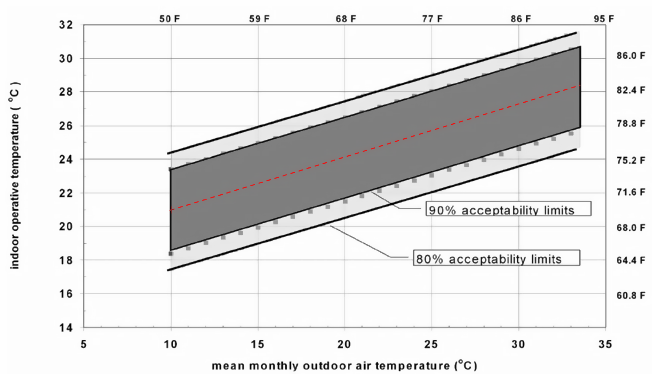
\includegraphics[width=0.9\textwidth, height=0.9\textheight, keepaspectratio=true]{media/image6814.png}
\caption{Acceptable operative temperature ranges for naturally conditioned spaces (ASHRAE Standard 55-2010) \protect \label{fig:acceptable-operative-temperature-ranges-for}}
\end{figure}

The central line of the model (shown in red), or comfort temperature, is defined as

\begin{equation}
{T_{ot}} = 0.31\cdot {T_o} + 17.8
\end{equation}

where:

T\(_{ot}\) is the operative temperature (\(^{\circ}\)C), calculated as the average of the indoor air dry-bulb temperature and the mean radiant temperature of zone inside surfaces

T\(_{o}\) is the monthly mean outdoor air dry-bulb temperature (\(^{\circ}\)C).

If the .stat file is provided for the simulation, T\(_{o}\) is drawn directly from the daily average temperatures in the .stat file, which provides a value for each month.~ If no .stat file is provided, the monthly mean outdoor temperature is a simple running average of the previous thirty daily average temperatures, calculated directly from the weather file (.epw):

\begin{equation}
{T_o} = \frac{{\left( {{T_{od - 1}} + {T_{od - 2}} + ... + {T_{od - 30}}} \right)}}{{30}}
\end{equation}

\begin{equation}
{T_o} = (1 - \alpha )\cdot {T_{od - 1}} + \alpha \cdot {T_{od - 1}}
\end{equation}

\begin{equation}
\alpha  = \frac{{29}}{{30}}
\end{equation}

T\(_{od-i}\) is defined as the daily average temperature of the i\(^{th}\) previous day.

Note that the weather file must be a standard .epw containing a full year of data.

The comfort regions for 80\% and 90\% acceptability are symmetric about the central line.

For 90\% Acceptability Limits:

\begin{equation}
T_{ot} = 0.31* T_{o} + 17.8 ± 2.5
\end{equation}

80\% Acceptability Limits:

\begin{equation}
T_{ot} = 0.31* T_{o} + 17.8 ± 3.5
\end{equation}

If, using either method, T\(_{o}\) is less than 10\(^{\circ}\)C or greater than 33.5\(^{\circ}\)C, the model is not applicable.

For a detailed description of this model, please see \emph{ASHRAE Standard 55-2010, Thermal Environmental Conditions for Human Occupancy}.

\subsection{Adaptive Comfort Model Based on European Standard EN15251-2007}\label{adaptive-comfort-model-based-on-european-standard-en15251-2007}

The EN15251-2007 is similar to ASHRAE 55-2010, but with slightly different curves of the indoor operative temperature and acceptability limits (Fig. 2). The model, intended for use in naturally ventilated buildings, determines the acceptability of indoor conditions given the 7-day weighted mean outdoor air temperature and the indoor operative temperature. The 7-day weighted mean outdoor air temperature (T\(_{rm}\)) is defined as the weighted running average of the previous 7 daily average outdoor air temperatures.

This weighted running average is calculated from a full annual weather file that must be specified for the simulation. This is used as an index for occupant adaptation to outdoor conditions, and determines the acceptability of indoor conditions. The model also accounts for people's clothing adaptation in naturally conditioned spaces by relating the acceptable range of indoor temperatures to the outdoor climate, so it is not necessary to estimate the clothing values for the space. No humidity or air-speed limits are required when this option is used. The model defines three comfort regions: Category I (90\%) Acceptability, Category II (80\%) Acceptability, and Category III (65\%) Acceptability. If T\(_{rm}\) is not within the specified domain of 10.0 to 30.0C, the model is not applicable.

\begin{figure}[hbtp] % fig 303
\centering
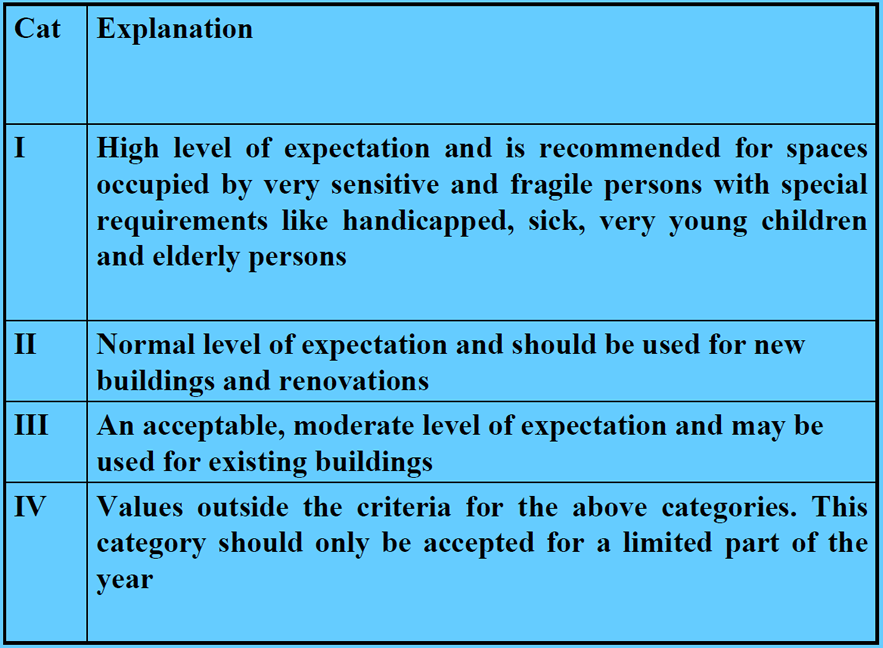
\includegraphics[width=0.9\textwidth, height=0.9\textheight, keepaspectratio=true]{media/image6819.png}
\caption{Categories for European Standard EN15251-2007 \protect \label{fig:categories-for-european-standard-en15251-2007}}
\end{figure}

\begin{figure}[hbtp] % fig 304
\centering
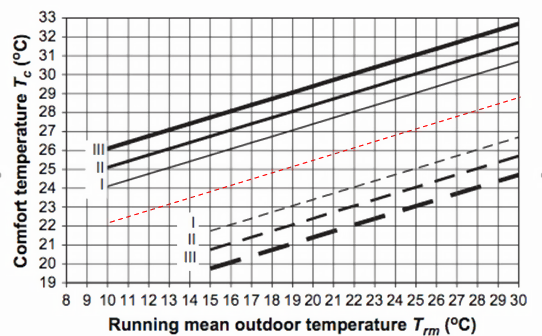
\includegraphics[width=0.9\textwidth, height=0.9\textheight, keepaspectratio=true]{media/image6820.png}
\caption{Acceptable operative temperature ranges for naturally conditioned spaces (CEN EN15251-2007) \protect \label{fig:acceptable-operative-temperature-ranges-for-001}}
\end{figure}

For the central line (shown as red in Figure~\ref{fig:acceptable-operative-temperature-ranges-for-001}):

\begin{equation}
T_{ot} = 0.33*T_o + 18.8
\end{equation}

For Category I, 90\% Acceptability Limits:

\begin{equation}
T_{ot} = 0.33*T_o + 18.8 \pm 2.0
\end{equation}

For Category II, 80\% Acceptability Limits:

\begin{equation}
T_{ot} = 0.33*T_o + 18.8 \pm 3.0
\end{equation}

For Category III, 65\% Acceptability Limits:

\begin{equation}
T_{ot} = 0.33*T_o + 18.8 \pm 4.0
\end{equation}

For 10\(^{\circ}\)C \textless{} T\(_{rm}\) \textless{} 15\(^{\circ}\)C, the comfort temperature of the lower boundaries of the comfort regions is T\(_{comf}\) = 23.75\(^{\circ}\)C. That is, the lower boundaries are constant according to the same ranges above:

For Category I, 90\% Acceptability Limits:

\begin{equation}
T_{ot} = 23.75 - 2.0
\end{equation}

For Category II, 80\% Acceptability Limits:

\begin{equation}
T_{ot} = 23.75 - 3.0
\end{equation}

For Category III, 65\% Acceptability Limits:

\begin{equation}
T_{ot} = 23.75 - 4.0
\end{equation}

where:

\({T_{ot}}\) is the operative temperature calculated as the average of the indoor air dry-bulb temperature and the mean radiant temperature of zone inside surfaces (\(^{\circ}\)C)

\(T_o\) is the mean outdoor air dry-bulb temperature (\(^{\circ}\)C), calculated as the weighted mean of the previous 7-day daily mean outdoor air dry-bulb temperature (T\(_{od}\)) using:

\begin{equation}
T_{o} = (1 - \alpha) * \{T_{od-1} + \alpha * T_{od-2} + \alpha^{2} * T_{od-3} + \alpha^{3} * T_{od-4} + \alpha^{4} * T_{od-5} + \alpha^{5} * T_{od-6} + \alpha^{6} * T_{od-7}\}
\end{equation}

\begin{equation}
T_{o} = (1 - \alpha) * T_{od-1} + \alpha * T_{o-1}
\end{equation}

\begin{equation}
\alpha = 0.8
\end{equation}

\subsection{Dynamic Clothing Model}\label{dynamic-clothing-model}

In most building energy simulations, thermal comfort condition is calculated based on the assumption that the clothing insulation is equal to a constant value of 0.5 clo during the cooling season and 1.0 clo during heating season. Usually those two values are used and the change from 0.5 to 1 or vice-versa is made suddenly from one day to another. In addition, there is no standardized guideline on how to set clothing insulation schedules in the international standards. This simplified assumption may lead to systems that are incorrectly sized and operated and to the incorrect assessment of comfort conditions. In reality, occupants frequently adjust their clothing depending on the thermal conditions around them, as opposed to the assumption of constant clothing values. Therefore, the clothing insulation variation should be captured during the building simulation to realistically model HVAC systems. In order to overcome the limitations of the constant clothing insulation assumption, three new predictive clothing insulation models were developed by Schiavon and Lee (2012) based on 6,333 selected observations taken from ASHRAE RP-884 and RP-921 databases. The first and third models vary the clothing insulation as a function of outdoor air temperature measured at 6 o'clock and the second model takes into account both 6 o'clock outdoor air temperature and indoor operative temperature when adjusting the clothing insulation. The dynamic clothing models should be implemented in dynamic building energy simulation.

The model proposed to ASHRAE 55 is described below.

For t\(_{a(out,6)}\) \textless{} -5\(^{\circ}\)C:

\begin{equation}
{I_{cl}} = 1.00
\end{equation}

For -5\(^{\circ}\)C \(\leq\) \(t_{a(out,6)}\) \textless{} 5\(^{\circ}\)C:

\begin{equation}
{I_{cl}} = 0.818 - 0.0364{\rm{*}}{t_{a\left( {out,6} \right)}}
\end{equation}

For 5\(^{\circ}\)C \(\leq\) t\(_{a(out,6)}\) \textless{} 26\(^{\circ}\)C:

\begin{equation}
{I_{cl}} = {10^{\left( { - 0.1635 - 0.0066{\rm{*}}{t_{a\left( {out,6} \right)}}} \right)}}
\end{equation}

Or for t\(_{a(out,6)}\) \(\geq\) 26\(^{\circ}\)C:

\begin{equation}
{I_{cl}} = 0.46
\end{equation}

where \(I_{cl}\) is the clothing insulation value and \(t_{a(out,6)}\) is the outdoor air temperature measured at 6 o'clock in the morning. Figure~\ref{fig:graphical-representation-of-the-proposed} illustrates the proposed clothing insulation model.

\begin{figure}[hbtp] % fig 305
\centering
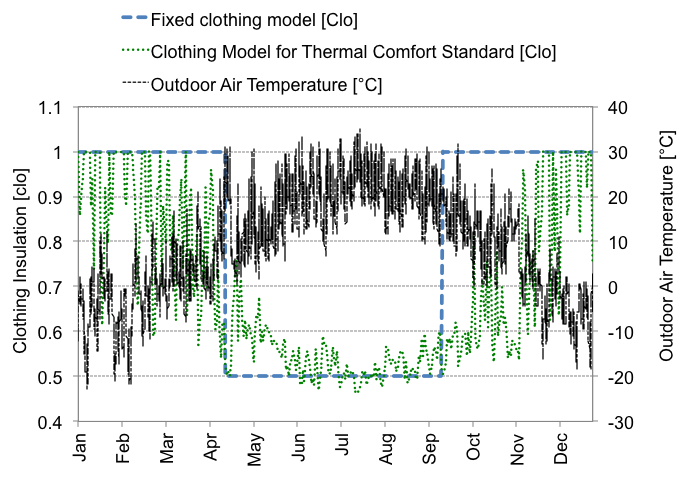
\includegraphics[width=0.9\textwidth, height=0.9\textheight, keepaspectratio=true]{media/image6825.png}
\caption{Clothing Schedule Illustration \protect \label{fig:clothing-schedule-illustration}}
\end{figure}

In Figure~\ref{fig:clothing-schedule-illustration}, clothing insulation schedule for a fixed model (blue) typically used in energy simulation software and for the clothing model based on outdoor air temperature measured at 6 o'clock. Climate data for Chicago O'hare International Airport has been used.

\begin{figure}[hbtp] % fig 306
\centering
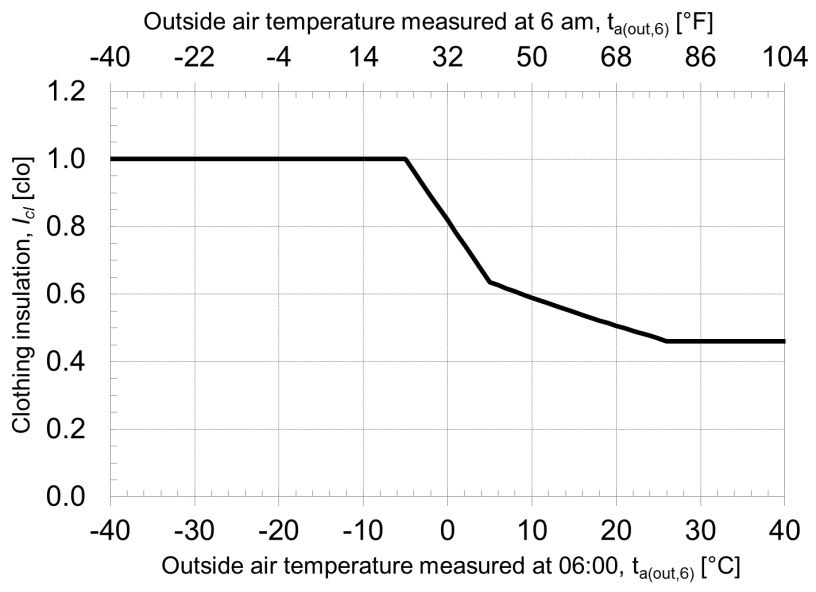
\includegraphics[width=0.9\textwidth, height=0.9\textheight, keepaspectratio=true]{media/image6826.png}
\caption{Graphical representation of the proposed clothing insulation model \protect \label{fig:graphical-representation-of-the-proposed}}
\end{figure}

The dynamic predictive clothing insulation model is implemented into EnergyPlus for realistic energy simulation. Addenda A to ASHRAE 55 with the clothing model has been approved by the ASHRAE committee and the chance to be included in ASHRAE 55-2013 is high.

\subsubsection{References}\label{references-033}

Schiavon S, Lee KH. 2013. Dynamic predictive clothing insulation models based on outdoor air and indoor operative temperatures. Building and Environment. Volume 59, 250-260. \url{http://dx.doi.org/10.1016/j.buildenv.2012.08.024} ~(link to the journal) \url{http://escholarship.org/uc/item/3338m9qf} ~(link to the freely available pre-print version)

Lee KH, Schiavon S. 2013. Influence of three dynamic predictive clothing insulation models on building energy use, HVAC sizing and thermal comfort. Submitted to Journal. \url{http://escholarship.org/uc/item/3sx6n876}~ (link to the freely available pre-print version)

\subsection{Mean Radiant Temperature Calculation}\label{mean-radiant-temperature-calculation}

There are three options to calculate mean radiant temperature in the thermal comfort models. One is the zone averaged MRT, another is the surface weighted MRT, and the other is angle factor MRT. The zone averaged MRT is calculated on the assumption that a person is in the center of a space, whereas the surface weighted MRT is calculated in consideration of the surface that a person is closest to, and the angle factor MRT is calculated based on angle factors between a person and the different surfaces in a space. Here, the surface weighted MRT is the average temperature of the selected surface and zone averaged MRT for the remaining surfaces in the zone and is intended to represent conditions in the limit as a person gets closer and closer to a particular surface.~ In that limit, half of the person's radiant field will be dominated by that surface and the other half will be exposed to the rest of the zone.~ Note that the surface weighted MRT is only an approximation. The angle factor MRT is the mean temperature of the surrounding surface temperatures weighted according to the magnitude of the respective angle factors and allows the user to more accurately predict thermal comfort at a particular location within a space.

% table 84
\begin{longtable}[c]{p{1.2in}p{2.0in}p{0.8in}p{0.8in}}
\caption{Nomenclature and variable list for MRT calculation \label{table:nomenclature-and-variable-list-for-mrt}} \tabularnewline
\toprule 
Mathematical variable & Description & Units ~ & Range
\tabularnewline
\midrule
\endfirsthead

\caption[]{Nomenclature and variable list for MRT calculation} \tabularnewline
\toprule 
Mathematical variable & Description & Units ~ & Range  
\tabularnewline
\midrule
\endhead

T\(_{r}\) & Mean radiant temperature & \(^{\circ}\)C & - \tabularnewline
T\(_{r-avg}\) & Zone averaged radiant temperature & \(^{\circ}\)C & -  \tabularnewline
T\(_{surf}\) & Surface temperature & \(^{\circ}\)C & -  \tabularnewline
F\(_{surf}\) & Angle factor between person and surface & - & 0-1  \tabularnewline
A\(_{surf}\) & Area of the surface & m\(^{2}\) & - \tabularnewline
\(\epsilon_{surf}\) & Emissivity of the surface & - & - \tabularnewline
\bottomrule
\end{longtable}

\subsubsection{Description of the model and algorithm}\label{description-of-the-model-and-algorithm-3}

The radiant temperature for the "zone averaged" option is simply calculated from the zone mean radiant temperature (MRT) without weighting any surface temperature of the zone more than the standard MRT calculation.

\begin{equation}
{T_r} = {T_{r - avg}}
\end{equation}

where the standard MRT is calculated using the following equation summed over all zone surfaces:

\begin{equation}
{T_{r - avg}} = \frac{\sum{{{\epsilon}_{i}}{{A}_{i}}{{T}_{i}}}}{\sum{{{\epsilon}_{i}}{{A}_{i}}}}
\end{equation}

In the surface weighted option, the radiant temperature is the average temperature of the modified zone averaged MRT and the temperature of the surface that a person is closest to.

\begin{equation}
{T_r} = ({T_{r - avg*}} + {T_{surf}})/2
\end{equation}

where the modified zone averaged MRT is calculated the same way as the standard MRT except that the surface closest to the person is left out of the summation:

\begin{equation}
{T_{r - avg*}} = \frac{\sum{{{\epsilon}_{i*}}{{A}_{i*}}{{T}_{i*}}}}{\sum{{{\epsilon}_{i*}}{{A}_{i*}}}}
\end{equation}

where when i is equal to the surface being used for weighting it is not included in either summation.

When the angle factor option is requested, the radiant temperature is the mean value of surrounding surface temperatures weighted by the surface emissivity, the size of the respective angle factors between a person and each surface, and the temperature to the fourth power for the surface.

\begin{equation}
{T_r} = \frac{\sum{{\epsilon_{i}}{F_{i}}{\PB{{T_{i}}}^4}}}{\sum{{\epsilon_{i}}{F_{i}}}}
\end{equation}

If all surfaces have the same emissivity that is close to unity, the emissivities in the above equation can be ignored.  However, since this is not always the case, the emissivity terms must be included in the above equation.  In addition, the temperatures to the fourth power in the above equation could be simplified to linear temperatures when the temperatures of the surfaces are fairly close.  However, as these temperatures get further apart, this linear approximation becomes increasingly poor.  As a result, since there is no guarantee that inside face surface temperatures will be close, the fourth order temperature terms are used to calculate the radiant temperature.

\subsection{References}\label{references-1-012}

ASHRAE. 1984. ``High Intensity Infrared Radiant Heating'', 1984 Handbook of Systems and Equipment, American Society of Heating, Refrigerating and Air Conditioning Engineers, Atlanta, GA, Chapter 18.

ASHRAE. 1985. ``Physiological Principles for Comfort and Health,'' 1985 Handbook of Fundamentals, American Society of Heating, Refrigerating and Air Conditioning Engineers, Atlanta, GA, Chapter 8.

ASHRAE. 1993. ``Physiological Principles and Thermal Comfort'', 1993 ASHRAE Handbook of Fundamentals, American Society of Heating, Refrigerating and Air Conditioning Engineers, Atlanta, GA, Chapter 8.

ASHRAE. 2010. ``Standard 55-2010 -- Thermal Environmental Conditions for Human Occupancy (ANSI approved)'', American Society of Heating, Refrigerating and Air Conditioning Engineers, Atlanta, GA.

Azer, N.Z., Hsu, S. 1977. ``The prediction of Thermal Sensation from Simple model of Human Physiological Regulatory Response'', ASHRAE Trans., Vol.83, Pt 1.

Berglund, Larry. 1978. ``Mathematical Models for Predicting the Thermal Comfort Response of Building Occupants'', ASHRAE Trans., Vol.84.

Doherty, T.J., Arens, E. 1988. ``Evaluation of the Physiological Bases of Thermal Comfort Models'', ASHRAE Trans., Vol.94, Pt 1.

Du Bois, D. and E.F. 1916. ``A Formula to Estimate Approximate Surface Area, if Height and Weight are Known'', Archives of internal Medicine, Vol.17.

CEN. 2007. ``Standard EN15251 Indoor environmental input parameters for design and assessment of energy performance of buildings addressing indoor air quality, thermal environment, lighting and acoustics''. Bruxelles: European committee for Standardisation.

Fanger, P.O. 1970. Thermal Comfort-Analysis and Applications in Environmental Engineering, Danish Technical Press, Copenhagen.

Fanger, P.O. 1986. ``Radiation and Discomfort'', ASHRAE Journal. February 1986.

Fanger P.O. 1967. ``Calculation of Thermal Comfort: Introduction of a Basic Comfort Equation'', ASHRE Trans., Vol.73, Pt 2.

Fountain, Marc.E., Huizenga, Charlie. 1997 ``A Thermal Sensation Prediction Tool for Use by the Profession'', ASHRAE Trans., Vol.103, Pt 2.

Gagge, A.P., Stolwijk, J. A. J., Nishi, Y. 1970. ``An Effective Temperature Scale Based on a Simple Model of Human Physiological Regulatory Response'', ASHRAE Trans., Vol.70, Pt 1.

Gagge, A.P., Fobelets, A.P., Berglund, L. G. 1986. ``A Standard Predictive Index of Human Response to the Thermal Environment'',~ ASHRAE Trans., Vol.92, Pt 2.

Hsu, S. 1977. ``A Thermoregulatory Model for Heat Acclimation and Some of its Application'', Ph. D. Dissertation, Kansas State University.

Int-Hout, D. 1990. ``Thermal Comfort Calculation / A Computer Model'', ASHRAE Trans., Vol.96, Pt 1.

ISO. 1983. ``Determination of the PMV and PPD Indices and Specification of the Conditions for Thermal Comfort'', DIS 7730, Moderate Thermal Environment, 1983.
